\documentclass[
  11pt,
  oneside,
  english,
  singlespacing,
  headsepline,
]{MastersDoctoralThesis}

\usepackage[utf8]{inputenc}
\usepackage[T1]{fontenc}
\usepackage{mathpazo}
\usepackage{amsmath}
\usepackage{graphicx}
\usepackage{minted}

\usepackage[backend=biber,style=apa,natbib=true]{biblatex}
\usepackage{caption}
\addbibresource{refs.bib}

\usepackage[autostyle=true]{csquotes}
\usepackage{tcolorbox}

\BeforeBeginEnvironment{minted}{\begin{tcolorbox}}%
\AfterEndEnvironment{minted}{\end{tcolorbox}}%

\geometry{
	paper=a4paper,
	inner=2.5cm,
	outer=3.8cm,
	bindingoffset=.5cm,
	top=1.5cm,
	bottom=1.5cm,
}

\thesistitle{Unlocking Biomedical Data for AI Health Research in Africa Using GeneNetwork as an Example}
\supervisori{Dr. Joseph \textsc{Sevilla}}
\supervisorii{Dr. Pjotr \textsc{Prins}}
\supervisoriii{Dr. Shelby \textsc{Solomon}}
\supervisoriv{Dr. George \textsc{Githinji}}
\examiner{}
\degree{Msc. Data Science And Analytics}
\author{\href{https://bonfacemunyoki.com}{Bonface Munyoki Kilyungi}}
\addresses{}

\keywords{Artificial Intelligence, Data Accessibility, Data Interpretation, GeneNetwork, Biological Data, Data Discovery, Resource Description Framework (RDF), Metadata} % Keywords for your thesis, this is not currently used anywhere in the template, print it elsewhere with \keywordnames
\university{\href{http://www.strathmore.edu}{Strathmore University}}
\department{\href{http://www.ilabafrica.ac.ke/}{iLab Africa}}
\faculty{} % Your faculty's name and URL, this is used in the title page and abstract, print it elsewhere with \facname

\AtBeginDocument{
\hypersetup{pdftitle=\ttitle} % Set the PDF's title to your title
\hypersetup{pdfauthor=\authorname} % Set the PDF's author to your name
\hypersetup{pdfkeywords=\keywordnames} % Set the PDF's keywords to your keywords
}

\begin{document}

% Use roman page numbering style (i, ii, iii, iv...) for the
% pre-content pages
\frontmatter

% Default to the plain heading style until the thesis style is called
% for the body content
\pagestyle{plain}

\begin{titlepage}
\begin{center}

\vspace*{.06\textheight}
%{\scshape\LARGE \univname\par}\vspace{1.1cm} % University name

\includegraphics[scale=0.5]{Logo}\\ % University/department logo - uncomment to place it
\textsc{\Large Dissertation Proposal}\\[0.5cm] % Thesis type

\HRule \\[0.4cm] % Horizontal line
{\huge \bfseries \ttitle\par}\vspace{0.4cm} % Thesis title
\HRule \\[1.5cm] % Horizontal line

\begin{minipage}[t]{0.4\textwidth}
\begin{flushleft} \large
% Author name - remove the \href bracket to remove the link
\emph{Author:}\\
\href{https://bonfacemunyoki.com}{\authorname} \\
\emph{Adm No:} 070707
\end{flushleft}
\end{minipage}
\begin{minipage}[t]{0.4\textwidth}
  \begin{flushright} \large
    \emph{Supervisors:} \\
    \supnamei\\
    \supnameii\\
    \supnameiii\\
    \supnameiv
\end{flushright}
\end{minipage}\\

\vfill

\large \textit{A dissertation submitted in fulfilment of the
  requirements\\ for Msc. Data Science and Analytics}\\[1cm]
% \deptname\\[1cm] % Research group name and department name

\noindent Approved by: \supnamei\\[1cm]
\noindent Signed:
\rule[0pt]{25em}{0.5pt}\\[1cm] % This prints a line for the signature

\noindent Date:
\rule[0pt]{25em}{0.5pt} % This prints a line to write the date
%% \vfill
%%     {\large \today}\\[4cm]


\end{center}

\end{titlepage}

%----------------------------------------------------------------------------------------
%	QUOTATION PAGE
%----------------------------------------------------------------------------------------

\vspace*{0.2\textheight}

\noindent\enquote{\itshape Life is like a pencil that will surely run out, but will leave the beautiful writing of life.}\bigbreak

\hfill Anonymous

%----------------------------------------------------------------------------------------
%	ABSTRACT PAGE
%----------------------------------------------------------------------------------------
\begin{abstract}
\addchaptertocentry{\abstractname} % Add the abstract to TOC

This dissertation aims to improve the accessibility and interpretability of biological data stored in the GeneNetwork (GN) repository for machine analysis.  The GN database contains over 20 years of experimental data from genetics, phenotyping, QTL, and GWA studies in human and model species, such as mouse and rat.  However, the data is currently difficult to access and manipulate due to its complex underlying structures, including around 80 cross-referenced SQL tables and various file types.  To address these challenges, this dissertation proposes to reorganize the data and provide automated data discovery using graph database technology.  This will enable the creation of a new, more flexible GN service and the ability to automatically infer relationships between data elements.  Overall, the expected outcome of this project is to enhance the value of the GN service through improved data retrieval and to allow for complex query capabilities and to map out future storage and retrieval techniques that are relevant for AI research on biomedical data.

\textbf{\textsc{Keywords:}} \textit{\keywordnames}
\end{abstract}


%----------------------------------------------------------------------------------------
%	LIST OF CONTENTS/FIGURES/TABLES PAGES
%----------------------------------------------------------------------------------------
\tableofcontents
%% \listoffigures
%% \listoftables

%----------------------------------------------------------------------------------------
%	ABBREVIATIONS
%----------------------------------------------------------------------------------------
% Include a list of abbreviations (a table of two columns)
\begin{abbreviations}{ll}
  \textbf{AI} & \textbf{A}rtificial \textbf{I}ntelligence\\
  \textbf{API} & \textbf{A}pplication \textbf{P}rogramming \textbf{I}nterface\\
  \textbf{DBMS} & \textbf{D}atabase \textbf{M}anagement \textbf{S}ystem\\
  \textbf{EMBL} & \textbf{E}uropean \textbf{M}olecular \textbf{B}iology \textbf{L}aboratory\\
  \textbf{GN} & \textbf{G}ene\textbf{N}etwork\\
  \textbf{GO} & \textbf{G}ene \textbf{O}ntology\\
  \textbf{GWA} & \textbf{G}enome-\textbf{W}ide \textbf{A}ssociation\\
  \textbf{HPO} & \textbf{H}uman \textbf{P}henotype \textbf{O}ntology\\
  \textbf{HTTP} & \textbf{H}yper\textbf{T}ext \textbf{T}ransfer \textbf{P}rotocol\\
  \textbf{NCBI} & \textbf{N}ational \textbf{C}enter for \textbf{B}iotechnology \textbf{I}nformation\\
  \textbf{QTL} & \textbf{Q}uantitative \textbf{T}rait \textbf{L}ocus\\
  \textbf{RDBMS} & \textbf{R}elational \textbf{D}atabase \textbf{M}anagement \textbf{S}ystem\\
  \textbf{RDF} & \textbf{R}esource \textbf{D}escription \textbf{F}ramework\\
  \textbf{SPARQL} & \textbf{S}PARQL \textbf{P}rotocol \textbf{A}nd \textbf{R}DF \textbf{Q}uery \textbf{L}anguage\\
  \textbf{SQL} & \textbf{S}tructured \textbf{Q}uery \textbf{L}anguage\\
  \textbf{URI} & \textbf{U}niform \textbf{R}esource \textbf{I}dentifier\\
  \textbf{W3C} & \textbf{W}orld Wide Web \textbf{C}onsortium\\
  
\end{abbreviations}


%----------------------------------------------------------------------------------------
%	DEDICATION
%----------------------------------------------------------------------------------------
\dedicatory{Dedicated to all the open source developers out there who fight for our freedoms through their efforts}


%----------------------------------------------------------------------------------------
%	THESIS CONTENT - CHAPTERS
%----------------------------------------------------------------------------------------
\mainmatter

\pagestyle{thesis}

\chapter{Introduction}
\label{chap:Introduction}
\section{Background}
Genetic data analysis is important for understanding the underlying mechanisms of various biological processes and diseases.  Genenetwork2 (\url{https://genenetwork.org}) is a powerful open-source software platform that provides a range of tools and resources for analysing, visualizing and storing genetic data, mostly written in the python programming language with a SQL database and flat files as a backend \citetext{\citealp{sloan2016genenetwork}; \citealp*{mulligan2017genenetwork}}.  It contains over 20 years of experimental data from genetics, phenotyping, QTL and GWA studies in human and model species such as mouse and rat \citep{sloan2016genenetwork}.  The size of the data is about 1TB and growing about 20\% a year.  The current SQL database underlying GN can be complex and difficult to write software against, and lacks interoperability with other systems.

The Resource Description Framework (RDF) is a widely-used graph based semantic data model that can provide several benefits over SQL, including support for complex data types, reasoning and ontologies \citep*{candan2001resource,allemang2011semantic}.  Representing GN's data in RDF has the potential to enable more flexible querying, data integration and reasoning capabilities, as well as better support for Linked Data and Semantic Web standards.  RDF is particularly suitable for machine learning and AI because it allows machines/software to analyse and discover the structure of the data and to start reasoning on it without human intervention.  So, by providing RDF, Genenetwork2 data will be easily accessible for AI.  This dissertation will make the data available for AI and make recommendations for future use of RDF in AI in a biological/clinical context.

\section{Problem Statement}

The current SQL database of Genenetwork2 has several limitations, such as its lack of support for complex data types, reasoning and ontologies.  These limitations make it difficult to integrate and query Genenetwork2's data with other sources and to perform advanced analysis tasks, such as inferencing and querying by example.

\section{General Objectives}

The main objective of this dissertation is to port Genenetwork2's SQL database to RDF, and to evaluate the benefits and challenges of this approach.

\section{Research Objectives}

\begin{enumerate}
\item To examine previous research and studies conducted on the GeneNetwork platform and Resource Description Framework (RDF).  
\item Understand the current limitations of the Genenetwork2 SQL database and how the use of RDF could address these limitations, as well as the potential benefits and challenges of porting the Genenetwork2 database to RDF, including its impact on data interoperability, integration and scalability.
\item Design, implement and test a framework for the porting process, including steps, tools and resources, for porting the Genenetwork2 database to RDF.
\item Validate the research by evaluating the benefits and challenges of the ported Genenetwork2 database in RDF, including its impact on data interoperability, integration and scalability.
\end{enumerate}

\section{Research Questions}

\begin{enumerate}
\item What are the previous studies and research work conducted on the GeneNetwork platform and RDF?
\item What are the current limitations of the Genenetwork2 SQL database and how could the use of RDF address these limitations?
\item How can we design, implement and test a framework for porting the Genenetwork2 database to RDF?
\item In the context of Genenetwork2, how does the performance of RDF compare against SQL/flat-files?
\end{enumerate}

\section{Research Relevance}

This dissertation aims to integrate RDF into the Genenetwork2 infrastracture, thereby facilitating a semantically enriched web environment that makes it easier to share data among various communities.  With the rise of Artificial Intelligence research, this dissertation creates a semantic infrastructure that will enable machines to autonomously analyse and discern data structures using inferencing techniques, eliminating the need for human intervention.  Consequently, this dissertation will contribute to the field of linked data storage, with a particular focus on the domains of biology and clinical research.

\section{Scope and Limitations}

The University of Tennessee Health Science Center will provide the dataset used in this dissertation.  Furthermore, access to one of their servers, capable of handling large databases at scale, will facilitate the work conducted in this dissertation.  Finally, this dissertation will not address any other issues or limitations related to Genenetwork2 beyond the current SQL database.


\chapter{Literature Review}
%To examine previous research and studies conducted on the GeneNetwork platform.
\section{GeneNetwork}
System genetics is a field of genetics that aims to understand how the interactions between genes, the environment, and other factors contribute to an organism's traits and characteristics.  GeneNetwork (\url{https://www.genenetwork.org}, GN) is a continuously updated web service for systems genetics analyses that allows researchers to analyze genetic data and identify patterns of covariation between different traits and genes \citep{mulligan2017genenetwork}.  It is a toolbox that allows for the analysis of genomic data in order to identify genetic associations with complex traits. The tool has been successfully used in a number of studies, including the expanded BXD family of mice cohort for experimental systems genetics and precision medicine \citep{Ashbrook:2019} and the GeneNetwork framework for web-based genetics \citep{sloan2016genenetwork}.  GN also allows for the upload of high-throughput experimental data, including genomic expression data obtained through microarray and RNA-sequencing technologies, as well as classical phenotypic data, such as disease-related traits \citep{Anderson:2021}.

GN is currently written in Python and JavaScript and comprises tooling and libraries that can be written in any computer language.  To guarantee bit for bit reproducibility and easy installation, the GN platform is packaged and deployed using GNU Guix \citep{sloan2016genenetwork}

While GN is a powerful platform for data integration and analysis, it has one major limitation in that it relies on a SQL database to retrieve metadata for specific experiments.  This metadata includes data from the PubMed database \footnote{https://www.ncbi.nlm.nih.gov/pubmed}, which is a widely used and comprehensive resource for scientific literature.  However, using PubMed  as a source of metadata for GeneNetwork may not provide the complete context for the relationships between the metadata and the data itself.  As shown with GeneCup, a tool for mining PubMed and the GWAS catalog for gene-keyword relationships, using the PubMed metadata without storing any of the relationships may not capture the full context of the relationships it identifies, potentially limiting the usefulness of the tool \citep{gunturkun2022genecup}.

\section{Linked Data and Semantic Web Standards}

Linked Data is a set of best practices for publishing and interlinking structured data on the Web \citep{bizer2011linkedData}.  It is based on the idea of using standard Web technologies, such as HTTP and RDF, to represent and link data in a way that is both human-readable and machine-readable.  Linked Data enables data from different sources to be connected and accessed in a decentralized manner, enabling data re-use and integration across a wide range of applications and domains \citep{bizer2011linkedData}.

\citep{lee2006exploring} proposed a set of principles for publishing data on the web in a way that enables data from different sources to be integrated into one single data space \citep{bizer2011linkedData}.  The rules/principles have become known as the \textit{``Linked Data principle''} and they are: (a) Use URIs as names for things; (b) Use HTTP URIs so that people can look up those names; (c) When someone looks up a URI, provide useful information, using the standards(RDF, SPARQL); and (d) include links to other URIs, so that they can discover more things \citep{bizer2011linkedData,lee2006exploring}.

The Semantic Web is a vision for the Web in which data is represented in a machine-readable form, enabling automated processing of Web content.  It is about making links, so that a person or machine can explore the web of data \citep{bizer2011linkedData}.  The Semantic Web relies on a set of standards, such as RDF and OWL, to represent and exchange data in a way that is both expressive and interoperable.  These standards provide a common vocabulary for data representation and enable the use of reasoning and inferencing to derive new knowledge from existing data.

The Semantic Web has several key properties which are important during application development.  One of these properties is that data is strictly separated from formatting and presentational aspects, which allows the data to be self-describing.  This implies that if an application using Linked Data encounters data with unfamiliar vocabulary, it can dereference the URIs that identify vocabulary terms to find their definition.  Additionally, use of HTTP as a standardised data access mechanism and RDF as standardised data model simplifies data access in comparison to Web APIs, which rely on heterogenous data models and access interfaces.  Furthermore, since the Semantic Web is open, applications do not have to be implmented against a fixed set of date \citep{bizer2011linkedData}.

In addition to their use in specific applications, Linked Data and Semantic Web standards have also been adopted as a general approach for improving data interoperability and enabling data integration.  For example, the Linked Data principles have been widely adopted by government agencies and other organizations as a way to publish and share data on the Web \citep{bizer2011linkedData}.  The use of Semantic Web standards has also been endorsed by the World Wide Web Consortium (W3C) as a way to enable the creation of a more interoperable and connected Web \citep{shadbolt2006semantic}.

\section{Resource Description Framework}
The Resource Description Framework (RDF) is a widely-used semantic data model that is designed to represent and exchange information about resources on the World Wide Web \citep{schreiber2014rdf}.  It is based on the idea of representing data as a set of triples, where each triple consists of a subject, predicate, and object.  The subject represents the resource being described, the predicate represents the property of the resource, and the object represents the value of the property \citep{schreiber2014rdf}.

RDF has several benefits for data modeling and representation, including its ability to support complex data types, reasoning, and ontologies \citep{schreiber2014rdf}.  One of the key benefits of RDF is its support for complex data types, such as lists, sets, and graphs.  This allows RDF to represent more complex relationships between resources, which is not possible with traditional data models such as relational databases \citep{allemang2011semantic}.

Another benefit of RDF is its support for reasoning, which is the process of inferring new information from existing data.  Reasoning can be used to make inferences about resources and their relationships, which can be particularly useful for data integration and querying \citep{allemang2011semantic}.

RDF also supports the use of ontologies, which are formal definitions of the concepts and relationships in a domain.  Ontologies provide a common vocabulary for data representation, which can improve data interoperability and facilitate data integration \citep{heath2011linked}.

One example of the use of RDF in genetics is the Gene Ontology (GO) project, which uses RDF to represent gene annotations and their relationships \citep{gene2004gene}.  The GO project has been widely adopted as a standard for gene annotation and is used by numerous databases and resources, including the European Molecular Biology Laboratory (EMBL) and the National Center for Biotechnology Information (NCBI).

Another example of the use of RDF in genetics is the Human Phenotype Ontology (HPO), which uses RDF to represent human phenotypes and their relationships \citep{robinson2010human}.  The HPO is a widely-used resource for annotating human phenotypes and has been used in numerous studies to support the analysis and interpretation of genetic data.

In the field of biomedical research, RDF has been used to represent and integrate data from multiple sources, including clinical trials and electronic health records \citep{luz2015providing}.  For example, a study published in the journal Health Informatics Journal used RDF to represent and integrate data from multiple sources, including clinical trials and electronic health records \citep{luz2015providing}.  The study demonstrated the feasibility of using RDF to represent and integrate complex data from multiple sources, and showed that RDF can support the integration and analysis of data from diverse domains.

There have also been numerous studies that have demonstrated the benefits of RDF for representing and integrating data in other domains, including biology, social media, and the Semantic Web \citep{schreiber2014rdf,allemang2011semantic,heath2011linked}.  These studies have shown that RDF can support the representation and integration of complex data from multiple sources, and can facilitate the use of reasoning and inferencing to derive new knowledge from existing data.

\section{SPARQL}

SPARQL (SPARQL Protocol and RDF Query Language) is a query language designed to retrieve and manipulate data stored in Resource Description Framework (RDF) format, which is a standard for representing data as a graph of interconnected triples\citep{prud2008sparql}.  It has become a popular choice for querying and integrating data from multiple sources, as it allows for the representation and integration of data from diverse domains, and the querying of that data using a single language.

One of the main advantages of SPARQL is its ability to query data from multiple sources and to combine data from those sources in a single query.  This is made possible through the use of federated queries, which allow SPARQL to query multiple RDF graphs or datasets in a single query \citep{allemang2011semantic,rakhmawati2013querying}.  This enables users to easily retrieve and integrate data from multiple sources, such as databases, ontologies, and web services, without the need to manually combine the data in a separate step.

Another advantage of SPARQL is its ability to handle complex queries and to perform operations such as aggregations and data transformation.  SPARQL includes a range of built-in functions and operators, as well as support for user-defined functions, which allow users to perform advanced operations on their data.  Additionally, SPARQL supports the use of subqueries, which allows users to nest queries within other queries, enabling the creation of highly sophisticated queries \citep{allemang2011semantic}.

According to \citep{allemang2011semantic}, SPARQL has been widely adopted in a variety of domains, including the Semantic Web, life sciences, and geospatial data management.  In the Semantic Web, SPARQL is often used to query linked open data sources, such as DBpedia and Wikidata, to retrieve and integrate data from multiple sources.  In the life sciences, SPARQL has been used to query biomedical ontologies and to integrate data from multiple sources, such as clinical trials and electronic health records.  In the geospatial domain, SPARQL has been used to query and integrate geospatial data from various sources, such as spatial databases and web services.

There are several implementations of SPARQL, including standalone servers, libraries for various programming languages, and web-based tools \citep{sparql22i}.  Some popular SPARQL implementations include Apache Jena, OpenRDF Sesame, and Virtuoso.

\section{SQL Databases and Their Limitations}
SQL databases are a type of database management system (DBMS) that are widely used for storing and manipulating structured data \citep{garcia2008database}.  Structured data is data that is organized into tables with rows and columns, and is well-suited for SQL databases because they provide efficient querying and data manipulation capabilities \citep{ramez2016fundamentals}.  However, SQL databases have certain limitations that can impact their performance and scalability \citep{chen2014data}.

One limitation of SQL databases is that they are not well-suited for storing large volumes of unstructured data, such as text documents or images \citep{chen2014data}.  While it is possible to store unstructured data in a SQL database, it requires additional processing and can be inefficient compared to using a database specifically designed for unstructured data, such as a NoSQL database \citep{kleppmann2019designing}.

Another limitation of SQL databases is that they do not scale well when dealing with large amounts of data or high levels of concurrency \citep{kleppmann2019designing,chen2014data}.  In order to scale a SQL database, it is necessary to partition the data across multiple servers or use techniques such as sharding, which can be complex and time-consuming to implement \citep{ramez2016fundamentals}.

SQL databases can also be limited in their ability to handle real-time data processing and analytics \citep{kleppmann2019designing,chen2014data}.  In order to perform real-time analysis on data stored in a SQL database, it is necessary to continuously update the database, which can impact performance and create additional overhead \citep{garcia2008database}.

\section{Summary}

SQL databases are a popular choice for storing structured data due to their efficient querying and data manipulation capabilities.  However, they have limitations when it comes to handling large volumes of unstructured data, scaling to handle large amounts of data or high levels of concurrency, and performing real-time data processing and analytics.  Linked Data and Semantic Web standards, such as RDF, provide a way to represent and exchange data in a machine-readable form, enabling automated processing and integration across a range of applications and domains.  RDF, in particular, allows for the representation of data as a set of interconnected triples, comprising a subject, predicate, and object.  This enables the creation of a graph-based data model that can be used to represent and link data on the Web.  SPARQL is a query language for RDF data that allows users to retrieve and manipulate data stored in an RDF graph.  It is commonly used in combination with Linked Data and Semantic Web technologies to enable the querying and integration of data from diverse sources.

\chapter{Methodology}

This chapter provides a comprehensive explanation of how each of the research questions listed in \Cref{chap:Introduction} will be addressed.  This involves showing how the proposed solution will be designed, how the research planning will be carried out and how development and testing will be done.

\section{Research Approach for Objectives 1 and 2}

The first objective of this dissertation was to study previous research work conducted on the GN platform and RDF.\@  Consequently, the second objective was focused on understanding the current limitations of the Genenetwork2 SQL database and exploring how the adoption of RDF could potentially address these constraints.  To meet these two objectives, a comprehensive literature review was conducted.

\section{Research Approach for Objectives 3}

In order to accomplish objectives three and four, a self-documenting Domain Specific Language (DSL) will be developed to facilitate the translation of SQL into RDF.\@  This DSL will be employed to convert SQL tables into RDF representations, subsequently enabling a comprehensive comparison of RDF performance against that of SQL\@.

The development methodology that will be adopted for this step is the \textit{Rapid Application Development (RAD)} methodology since it prioritizes development and prototype-building over planning.  It emphasizes the end-user involvement, prototyping, reuse and the use of automated tools \citep*{van2008software}.  This gives the researcher the ability to efficiently execute numerous iterations and updates to the software/model without the need to begin each iteration anew.  This yields a significant advantage, as it facilitates the ability to modify the design, augment functionality and iteratively refine the software/model at a high frequency.

\citet*{van2008software} outlines the four fundamental steps of the Rapid Application Development (RAD) methodology as:

\begin{enumerate}
\item \textbf{Requirements Planning:} In contrast to traditional software development models, the RAD methodology begins by obtaining a general understanding of the requirements rather than seeking a comprehensive list of specifications from end users.  The broad nature of the requirements allows for the segmentation of specific requirements at different points throughout the development cycle.

\item \textbf{Prototyping:} At this stage, actual development occurs.  Prototypes are created featuring various functionalities rapidly, deviating from a strict set of requirements.  Typically, these prototypes are hastily constructed to demonstrate key features.  The final software artifact is only developed during the finalization stage, where the consensus on the desired outcome has been reached.

\item \textbf{Construction:}  In this stage, the working model is transformed into a functional system.  Usually, most bugs, issues and modifications are addressed.

\item \textbf{Cutover:} The final stage of RAD involves the final testing of the system before the system is ready to use by end users.  The cutover phase encompasses intensive scale testing, technical documentation, issue tracking, final customizations and possible system simulations.
\end{enumerate}

Figure~\ref{fig:rad-lifecycle} shows the aforementioned RAD life-cycle.

\begin{figure}[H]
  \centering
  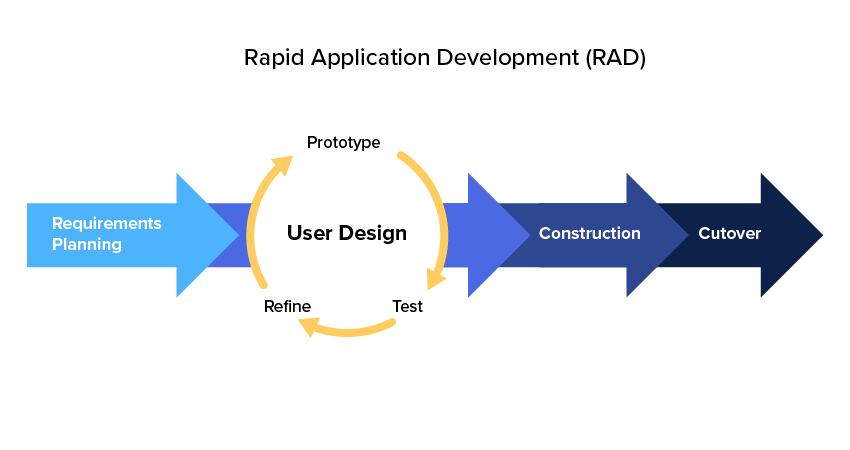
\includegraphics[width=12cm]{RAD}
  \caption{Rapid Application Development life-cycle}
  \source{https://kissflow.com/application-development/rad/rapid-application-development-rad-meaning/}\label{fig:rad-lifecycle}
\end{figure}

The following subsections elaborate on the application of the RAD methodology within this dissertation's context.

\subsection{Requirements Planning}

The process of requirements planning is the initial stage in building the DSL.\@  This stage encompasses activities such as conceptual ideation, during which potential representations of the DSL are brainstormed.  The primary goal is to design a self-documenting DSL that is comprehensible and accessible to human end-users.  Moreover, the DSL should support s-expressions and offer a declarative mapping of SQL query results to a predefined ontology.  Furthermore, in this stage, relevant public and active ontologies will be identified.  The DSL will use these ontologies when transforming data from SQL tables to RDF\@.

\subsection{Prototyping}

During the prototyping phase, a preliminary version of the DSL will be developed, enabling the exploration of its design and functionality.  This prototype will function as a proof-of-concept, subject to refinement through feedback from the GeneNetwork leadership team~\footnote{\url{https://git.genenetwork.org/gn-docs/tree/general/team/leadership.md}}, whose members possess extensive experience in programming, genetics, and genomics.  They were selected for their ability to evaluate RDF progress and offer valuable insights.  Figure~\ref{fig:parser-demo} illustrates the parser's basic operation.

\begin{figure}[H]
\centering
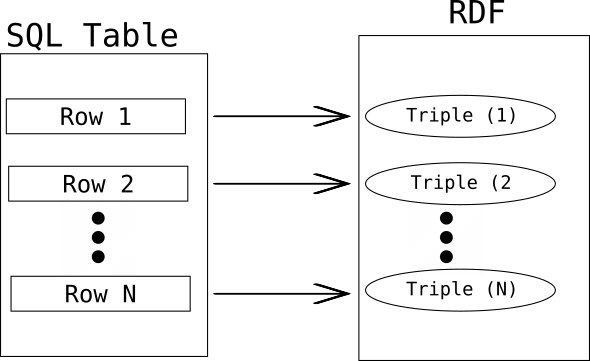
\includegraphics[width=8cm]{parserDemo}
\caption{\textit{The parser operates on each row to produce a valid triple store}}\label{fig:parser-demo}
\centering
\end{figure}

During the prototyping stage, it is crucial to quickly check whether syntactical errors exist in the RDF output.  To this end, \textit{rapper}~\footnote{\url{https://librdf.org/raptor/rapper.html}}, a Raptor RDF parser utility, will be utilized to assess the syntactic correctness of the generated RDF format.  This linting process ensures that the output is free of errors, permitting the data to be ingested into a virtuoso instance.  In the absence of errors detected during the linting procedure, the data can subsequently be uploaded to a running Virtuoso instance.

\subsection{Construction}

The construction phase encompasses the development of a robust, reusable tool.  During this stage, numerous unforeseen challenges, including bugs, issues, and modifications, will be identified and addressed.  In order to prevent regressions, tests will be implemented concurrently with the development process, ensuring the tool's reliability and functionality.

\subsection{Cut-off}

During this final stage, the Domain Specific Language (DSL) will be used to convert GeneNetwork tables into RDF format.  Components of GeneNetwork that rely extensively on metadata will be restructured to utilize RDF.\@  A comparison between SQL and RDF performance will be assessed.

\section{Validation}

The final objective of this dissertation is to validate this dissertation by comparing the performance of RDF against SQL/flat-files.  To validate the findings in this dissertation, performance benchmarks will be conducted to compare the efficiency of RDF, SQL and flat-files in different scenarios.  The performance benchmarks will include measuring the time required to execute specific queries.  Moreover, functionalities that can be achieved using SPARQL but not SQL will be identified.

%%% Local Variables:
%%% ispell-local-dictionary: "en_GB-ise"
%%% End:

\chapter{System Design and Architecture}

\section{Introduction}

This chapter presents a technical framework and architecture for implementing an embedded self-documenting DSL that is written in Scheme.  In addition to the DSL, this chapter will also different ontologies that will be used to model data.  The proposed DSL provides human-friendly syntax that allows a user to select tables from a SQL database, translate them into RDF, and save the output in a specified file, all while generating a markdown file that has documentation about that given dump.  Given the DSL's foundation in Scheme, end users are also able to leverage Scheme's capabilities within the DSL's framework, thereby enhancing its extensibility.

\section{Design Process}

\subsection{Design Goals}

In contrast to general-purpose languages (GPLs), DSLs present certain benefits, as highlighted by \citet{freudenthal2010domain} and \citet{spinellis2001notable}:

\begin{enumerate}
\item \textit{Explicit Representation of Domain Knowledge:} DSLs allow domain-specific functionality to be expressed in a tangible, human-readable format at a high level of abstraction.  This clarity makes software artifacts more accessible to developers, thereby simplifying the processes of development, testing and modification.
\item \textit{Active Engagement of Domain Experts:} Programs crafted in DSL often adopt a style that aligns with the conventional formats used by domain experts.  This facilitates their participation in the software's lifecycle and promotes collaboration with developers. In some cases, domain experts might directly specify, implement, verify or validate certain artifacts.
\end{enumerate}

In lieu of the aforementioned advantages of a DSL, the system architecture should accomplish the following:

\begin{enumerate}
\item The architecture must be \textit{database agnostic.}  Given that users will be employing this DSL with their unique databases, it is essential for the DSL to be flexible enough to support constructs that allows them to work with their unique database.
\item The architecture should empower users to model, in the context of some defined ontology, the mapping of the results derived from their SQL queries into RDF.
\item The DSL should provide a means of self-documenting itself while transforming data from SQL to RDF.
\end{enumerate}

\subsection{Architecture}
% How did you design your system
\begin{figure}[H]
  \centering
  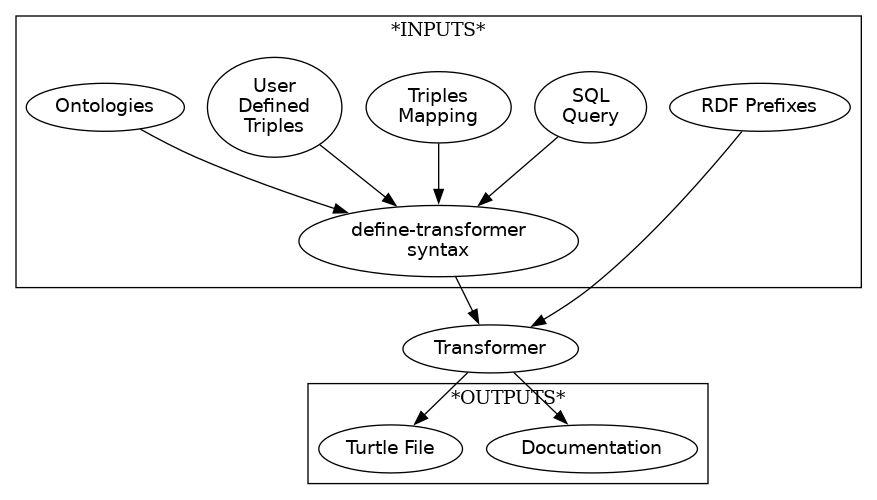
\includegraphics[width=12cm]{systemDesign}
  \caption{\textit{Overview of how SQL is converted to RDF and documentation}}
  \label{fig:layered-arch}
  \centering
\end{figure}

%% To achieve the design goals outlined above, the layered architectural pattern \citep{richards2015software} is used.  The DSL is organized into four primary layers:

%% \begin{enumerate}
%% \item The first layer encompasses the Input-Output operations related to a file.
%% \item The second layer embodies the processes of adding an RDF prefix and defining a dump that works on a single table.
%% \item The third layer portrays the semantic elements needed to define a dump.
%% \item The final layer illustrates the potential operations that can be nested when defining an RDF triple.
%% \end{enumerate}
    
%% The structure of these layers is visualized in Figure \ref{fig:layered-arch}.

%% \begin{figure}[H]
%%   \centering
%%   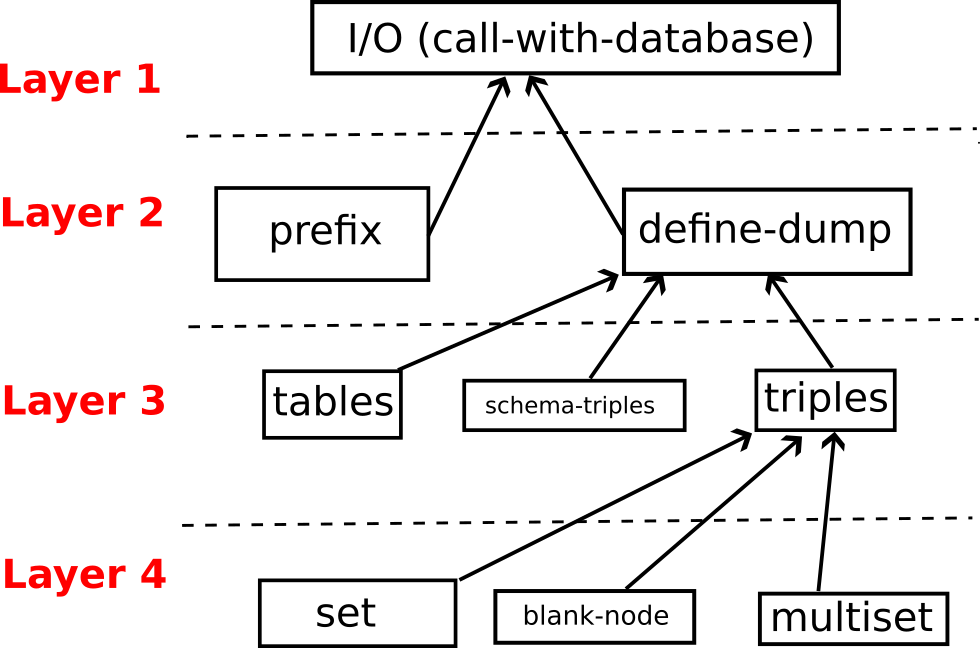
\includegraphics[width=12cm]{archLayers}
%%   \caption{\textit{Architecture layers}}
%%   \label{fig:layered-arch}
%%   \centering
%% \end{figure}

%% \subsubsection{Layer 1}

%% This layer contains the I/O operation: \textit{call-with-database}.  This allows a database connection that can be passed down to functions defined in the layers below it.

%% \subsubsection{Layer 2}

%% ``prefix'' allows the user to define a given RDF prefix, and ``define-dump'' allows them to model a given table that will be dumped.  ``define-dump'' depends on elements of Layer 3 to operate.

%% \subsubsection{Layer 3}
%% This layer is where most of the modelling happens.  All elements in this layer are composed together to form ``define-dump'' as follows:

%% The \texttt{tables} clause specifies the database tables to be joined to construct the view to be parsed.  \texttt{TABLE} can be in the form \texttt{TABLE-NAME} or of the form \texttt{JOIN-OPERATOR TABLE-NAME RAW-CONDITION}.  \texttt{TABLE-NAME} is the name of the target table.  The \texttt{JOIN-OPERATOR} can be either a join, left-join or an inner-join.  \texttt{RAW-CONDITION} is the join condition as a raw string, for example \texttt{``USING (SpeciesId)''}.  \texttt{RAW-FORMS} are expressions that should evaluate to strings which will be appended to the SQL query during macro-expansion.

%% The \texttt{schema-triples} clause identifies the list of triples written once when the dump begins.

%% The triples clause specifies the triples to be dumped once for each row in the view.  All triples have a common \texttt{SUBJECT}. The \texttt{(verb predicate object)} clauses are described below:

%% \begin{itemize}
%% \item \texttt{VERB} must either be a set or multiset. For the set \texttt{VERB}, a single triple \texttt{(SUBJECT PREDICATE OBJECT-VALUE)} is written where \texttt{OBJECT-VALUE} is the result of evaluating \texttt{OBJECT}. For the multiset \texttt{VERB}, \texttt{OBJECT} must evaluate to a list, and a triple \texttt{(SUBJECT PREDICATE OBJECT-VALUE-ELEMENT)} is created for each element \texttt{OBJECT-VALUE-ELEMENT} of that list.
%% \item The \texttt{SUBJECT} and \texttt{OBJECT} expressions in the triples clause must reference database fields using a \texttt{(field TABLE COLUMN)} clause where \texttt{TABLE} and \texttt{COLUMN} refer to the table and column of the field being referenced. Database fields can also be referenced using \texttt{(field TABLE COLUMN ALIAS)} where \texttt{ALIAS} is an alias for that column in the SQL query.
%% \end{itemize}

%% \subsubsection{Layer 4}

%% The ``triples'' from the previous layer can have a:

%% \begin{enumerate}
%% \item \textit{set:} represents a single element.
%% \item \textit{multiset:} represents multiple elements.
%% \item \textit {blank-node:} represents the concept of a blank-node which is a native RDF construct.
%% \end{enumerate}



%----------------------------------------------------------------------------------------
%	BIBLIOGRAPHY
%----------------------------------------------------------------------------------------
\printbibliography[heading=bibintoc]

\end{document}
